% Printed 103; principal PDF 110; Google PDF 114.
\par\clearpage

\vspace*{.09\textheight}
\begin{center}{\LARGE N\,A\,C\,H\,L\,A\,S\,S.}\end{center}
\vspace{.05\textheight}
\begin{center}
[1.]\\[.5ex]
Reduktion der sphärischen Dreieckswinkel \(A,B,C\) auf die Sehnenwinkel\\
\(\mathfrak{A},\mathfrak{B},\mathfrak{C}\).
\end{center}

\noindent\begin{minipage}[t]{.65\textwidth}
\setlength{\parindent}{1.5em}
\indent Man beschreibe um das Dreieck einen Kreis.\\
Also die 3 Vierecke das Maß [der Korrekturen].

Man mache
\[
\frac{a}{\sin A}=\frac{b}{\sin B}=\frac{c}{\sin C}=\nu
\]
\[
\nu a\cos A=\alpha,\quad \nu b\cos B=\beta,\quad \nu c\cos C=\gamma.
\]
\noindent Dann sind die Reduktionen
\[
\frac{\beta+\gamma}{8},\quad
\frac{\alpha+\gamma}{8},\quad
\frac{\alpha+\beta}{8}.
\]
\end{minipage}\hfill
\begin{minipage}[t]{.33\textwidth}
\vspace{0pt}\centering
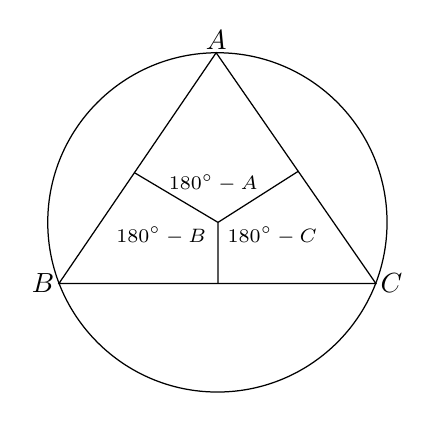
\begin{tikzpicture}[x=1.55cm,y=1.55cm,line width=.45pt]
\coordinate (A) at (-.01,1.39);
\coordinate (B) at (-1.298,-.50);
\coordinate (C) at (1.298,-.50);
\coordinate (O) at (.005,0);
\path (A)--(B) coordinate[pos=.52] (AB);
\path (A)--(C) coordinate[pos=.514] (AC);
\path (B)--(C) coordinate[pos=.502] (BC);
\draw (0,0) circle[radius=1.39];
\draw (A)--(B)--(C)--cycle;
\draw (AB)--(O)--(AC) (O)--(BC);
\node[above,inner sep=1pt] at (A) {\(A\)};
\node[left,inner sep=1.5pt] at (B) {\(B\)};
\node[right,inner sep=1.5pt] at (C) {\(C\)};
\node[font=\scriptsize,inner sep=0pt] at (-.035,.32) {\(180^\circ-\mathfrak A\)};
\node[font=\scriptsize,inner sep=0pt] at (-.46,-.11) {\(180^\circ-\mathfrak B\)};
\node[font=\scriptsize,inner sep=0pt] at (.45,-.11) {\(180^\circ-\mathfrak C\)};
\end{tikzpicture}
\end{minipage}
\par\bigskip

\begin{center}
[2.]\\[.5ex]
{[Bedingung dafür, dass 3 Punkte auf der Oberfläche einer Kugel}\\
auf einem Großkreis liegen.]
\end{center}

Die Bedingung dafür, dass drei Punkte auf der Oberfläche einer Kugel mit den jeweiligen Längen und
Breiten
\[
\begin{array}{l}
L,\ B\\
L',\ B'\\
L'',\ B''
\end{array}
\]
\noindent auf einem Großkreis liegen, lautet
\[
\operatorname{tang}B\sin(L'-L'')+\operatorname{tang}B'\sin(L''-L)+
\operatorname{tang}B''\sin(L-L')=0.
\]

\begin{center}\rule{.18\textwidth}{.4pt}\end{center}

% Printed 104; principal PDF 111; Google PDF 115.
\par\clearpage
\noindent\makebox[12mm][l]{\fontsize{13}{16}\selectfont 104}\makebox[\dimexpr\linewidth-24mm\relax][c]{\scriptsize\textbf{BEMERKUNGEN.\quad REDUKTION DER SPHÄRISCHEN DREIECKSWINKEL ETC.}}\makebox[12mm][r]{}\par\medskip

\vspace*{.11\textheight}
{\small
\begin{center}\textbf{BEMERKUNGEN.}\end{center}

Die Notiz [1] ist in ein Rechnungsheft für die hannoversche Gradmessung eingetragen. \textsc{Gauss} hat
hier als Werte der Korrekturen \(\frac{\beta+\gamma}{4}\), \(\frac{\alpha+\gamma}{4}\), \(\frac{\alpha+\beta}{4}\) angegeben. Die Reduktion von \(A\) auf \(\mathfrak A\) kann man
aus der Gleichung
\[
\cos\mathfrak A=\sin\frac b{2r}\sin\frac c{2r}
+\cos\frac b{2r}\cos\frac c{2r}\cos A,\quad (r=\text{Radius der Kugel})
\]
\noindent erhalten, deren Entwicklung zunächst
\[
A-\mathfrak A=\frac1{4rr}\,.\,\frac{bc}{\sin A}
-\frac1{8rr}(bb+cc)\operatorname{cotang}A\ldots
\]
\noindent liefert. Beschränkt man sich auf die Glieder zweiter Ordnung, so kann man
\[
bb+cc=aa+2bc\cos A
\]
\noindent setzen. Damit ergibt sich
\[
A-\mathfrak A=\frac1{8rr}(2bc\sin A-aa\operatorname{cotang}A)
=\frac1{8rr}(bb\operatorname{cotang}B+cc\operatorname{cotang}C).
\]
\noindent Zu demselben Ergebnis gelangt man, wenn man bedenkt, dass \(A-\mathfrak A\) gleich dem Exzess des sphärischen
Vierecks ist, dessen Eckpunkte der Pol des Dreiecks, die Fußpunkte der Lote von diesem auf die Seiten
\(b\) und \(c\) und der Punkt \(A\) sind.

Die Notiz [2] befindet sich auf dem letzten Blatt des \textsc{Gauss}schen Exemplars der »Analytischen
Trigonometrie von G. S. \textsc{Klügel}. Braunschweig 1770«. Nach einer Vorlesung, die \textsc{Gauss}
unter dem Titel »Anleitung zur höhern Geodäsie« hielt und von der eine Nachschrift vorliegt, beruht die Ableitung
der in [2] angegebenen Bedingungsgleichung darauf, dass aus
\[
\begin{aligned}
m&=n\sin(\varphi-\Phi)\\
m'&=n\sin(\varphi'-\Phi)\\
m''&=n\sin(\varphi''-\Phi)
\end{aligned}
\]
\noindent die Gleichung
\[
m\sin(\varphi'-\varphi'')+m'\sin(\varphi''-\varphi)+m''\sin(\varphi-\varphi')=0
\]
\noindent folgt. Bezeichnet nun \(i\) den Neigungswinkel der Ebene des Großkreises gegen die Äquatorebene und
werden die Längen \(L-L_0\), \(L'-L_0\), \(L''-L_0\) von dem Meridian an gezählt, der durch die Schnittlinie beider Ebenen verläuft,
so gilt
\[
\begin{aligned}
\operatorname{tang}B&=\operatorname{tang}i\sin(L-L_0)\\
\operatorname{tang}B'&=\operatorname{tang}i\sin(L'-L_0)\\
\operatorname{tang}B''&=\operatorname{tang}i\sin(L''-L_0).
\end{aligned}
\]
\par\hfill\textsc{Krüger, Börsch.}\hspace{.06\textwidth}\par
}
\begin{center}\rule{.24\textwidth}{.4pt}\end{center}

